\providecommand{\main}{../../..}
\documentclass[\main/main.tex]{subfiles}
\begin{document}

\subsection{Esercizio 2}
Dato il problema di programmazione matematica

\begin{align*}
  \min f(x) & =x^2_1+x^2_2           \\
  g_1(x)    & = 1-x_1x_2 \leq 0      \\
  g_2(x)    & = x_1 + x_2 -4 \leq 0  \\
  g_3(x)    & = -x_1 - x_2 - 2\leq 0
\end{align*}

\begin{enumerate}[a)]
  \item Si rappresenti il problema graficamente.
  \item Si determinino gli eventuali punti non regolari o si mostri che non ne esistono.
  \item Si determinino i punti candidati secondo le condizioni di KKT, e in particolare quello/i di minimo.
\end{enumerate}

\subsection{Soluzione esercizio 2}

\paragraph*{a) La funzione nel suo dominio di definizione è la seguente:}

\begin{figure}
  \begin{subfigure}{0.45\textwidth}
    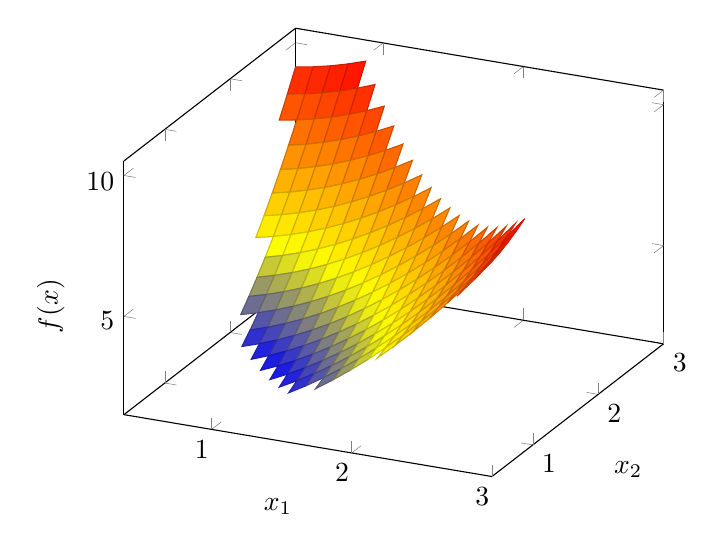
\begin{tikzpicture}
      \begin{axis}[
          xlabel=$x_1$,
          ylabel=$x_2$,
          zlabel=$f(x)$,
          domain=0:3,
          y domain=0:3
        ]
        \addplot3[surf, unbounded coords=jump]
        {1-x*y < 0 && x + y < 4 && -x - y < 2 ? y^2 + x^2 : NaN};
      \end{axis}
    \end{tikzpicture}
    \caption{La funzione $f(x)$}
  \end{subfigure}
  ~
  \begin{subfigure}{0.45\textwidth}
    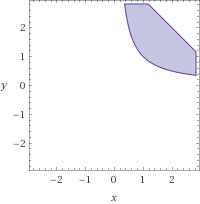
\includegraphics[width=0.8\textwidth]{11042016domain}
    \caption{Dominio della funzione $f(x)$}
  \end{subfigure}
\end{figure}

\paragraph*{Calcolo dei punti non regolari:}
Calcolo i gradienti dei vincoli:
\[
  \nabla g_1 = \begin{bmatrix}
    -x_2 \\
    -x_1
  \end{bmatrix}
  \qquad
  \nabla g_2 = \begin{bmatrix}
    1 \\
    1
  \end{bmatrix}
  \qquad
  \nabla g_3 = \begin{bmatrix}
    -1 \\
    -1
  \end{bmatrix}
\]

Il gradiente $ \nabla g_1$ si annulla nell'origine, che è all'esterno del dominio di interesse (nessun vincolo è attivo in quel punto). Gli altri gradienti $ \nabla g_2$ e $\nabla g_3$ non si annullano.

Calcolo i punti dati dall'intersezione dei vincoli a coppie:

\subparagraph*{Vincoli $g_1$ e $g_2$:}

\[
  \begin{cases}
    1-x_1x_2 = 0 \\
    x_1 + x_2 - 4 = 0
  \end{cases}
  \Rightarrow
  \begin{cases}
    1-x_2(4 - x_2) = 0 \\
    x_1  = 4 - x_2
  \end{cases}
  \Rightarrow
  \begin{cases}
    x^2_2 - 4x_2 +1 = 0 \Rightarrow x_2 = 2 \pm \sqrt{3} \\
    x_1  = 4 - x_2
  \end{cases}
\]

Da cui deriviamo i punti $A = (2 + \sqrt{3}, 2 - \sqrt{3})$ e $B = (2 - \sqrt{3}, 2 + \sqrt{3})$. In nessuno di questi punti la matrice realizzata accostando i gradienti risulta singolare, quindi i punti $A$ e $B$ sono regolari.

\subparagraph*{Vincoli $g_1$ e $g_3$:}

\[
  \begin{cases}
    1-x_1x_2 = 0 \\
    x_1  = -x_2 - 2
  \end{cases}
  \Rightarrow
  \begin{cases}
    1+x^2_2 +2x_2 = 0 \Rightarrow x_2 = 1 \\
    x_1  = -3
  \end{cases}
\]

Ne deriviamo il punto $C = (-3, 1)$ che nuovamente non annulla il determinante della matrice dei gradienti ed è quindi regolare.

\subparagraph*{Vincoli $g_2$ e $g_3$:}
I due vincoli non hanno intersezioni.

\subparagraph*{Vincoli $g_1$, $g_2$ e $g_3$:}
I tre vincoli non hanno intersezioni comuni.

\paragraph*{Condizioni KKT}
\subparagraph*{Calcolo della lagrangiana generalizzata}

\[
  l(x) = x^2_1+x^2_2 + \mu_1 (1-x_1x_2) + \mu_2 (x_1 + x_2 -4) + \mu_3 (-x_1 - x_2 - 2)
\]

\subparagraph*{Realizzo il sistema delle condizioni KKT}

\[
  \begin{cases}
    \nabla l(x) = \begin{bmatrix}
      2x_1 + \mu_1x_2 + \mu_2 + \mu_3 \\
      2x_2 + \mu_1x_1 + \mu_2 + \mu_3
    \end{bmatrix} = \bm{0} \\
    \mu_1 (1-x_1x_2) = 0                              \\
    \mu_2 (x_1 + x_2 -4) = 0                          \\
    \mu_3 (-x_1 - x_2 - 2) = 0                        \\
    1-x_1x_2 \leq 0                                   \\
    x_1 + x_2 -4 \leq 0                               \\
    -x_1 - x_2 - 2 \leq 0                             \\
    \mu_1 \geq 0                                      \\
    \mu_2 \geq 0                                      \\
    \mu_3 \geq 0                                      \\
  \end{cases}
  \Rightarrow
  \begin{cases}
    2x_1 + 2x_2 + \mu_2 + \mu_3 = 0 \\
    \mu_2 (x_1 + x_2 -4) = 0        \\
    \mu_3 (-x_1 - x_2 - 2) = 0      \\
    1-x_1x_2 = 0                    \\
    x_1 + x_2 -4 \leq 0             \\
    -x_1 - x_2 - 2 \leq 0           \\
    \mu_1 = 2                       \\
    \mu_2 \geq 0                    \\
    \mu_3 \geq 0                    \\
  \end{cases}
\]

\subparagraph*{Caso $\mu_2 = 0 \land g_2 \leq 0$}
\[
  \begin{cases}
    \mu_3 = -\frac{2}{x_2} - 2x_2  \Rightarrow \mu_3 = 3 \\
    (1 + x^2_2) (x_2+1)^2 = 0  \Rightarrow x_2 = -1      \\
    x_1 = \frac{1}{x_2}   \Rightarrow x_1 = -1           \\
    x_1 + x_2 -4 \leq 0       \Rightarrow -6 \leq 0      \\
    -x_1 - x_2 - 2 \leq 0 \Rightarrow  0 = 0             \\
    \mu_1 = 2                                            \\
    \mu_2 = 0                                            \\
    \mu_3 = 3                                            \\
  \end{cases}
\]

Viene identificato il punto candidato $D = (-1, -1)$.

\subparagraph*{Caso $\mu_2 > 0 \land g_2 = 0$}

\[
  \begin{cases}
    \mu_2 = -\frac{2}{2 \pm \sqrt{3}} - 2(2 \pm \sqrt{3})                        \\
    \mu_3 (1 + (2 \pm \sqrt{3})^2 + 2(2 \pm \sqrt{3})) = 0 \Rightarrow \mu_3 = 0 \\
    x_1 = \frac{1}{x_2}  \Rightarrow x_1 = \frac{1}{2 \pm \sqrt{3}}              \\
    1 + x^2_2 -4x_2 = 0  \Rightarrow x_2 = 2 \pm \sqrt{3}                        \\
    -x_1 - x_2 - 2 \leq 0                                                        \\
    \mu_1 = 2                                                                    \\
    \mu_2 > 0                                                                    \\
    \mu_3 = 0                                                                    \\
  \end{cases}
\]

I valori ottenuti non rispettano il vincolo $\mu_2 \geq 0$.

\paragraph*{Calcolo del valore dei punti candidati}

\[
  \begin{cases}
    f(A) = f(2+\sqrt3, 2 - \sqrt{3}) = 14  \\
    f(B) =  f(2-\sqrt3, 2 + \sqrt{3}) = 14 \\
    f(C) = f(-3, -1) = 10                  \\
    f(D) = f(-1, -1) = 2                   \\
  \end{cases}
\]

Il punto di ottimo locale risulta essere $D$.

\end{document}